%!TEX program = lualatex
\documentclass[bachelorthesis, grey, english]{mas-thesis-chapters} % Available options:
															     % masterthesis, bachelorthesis, dissertation
															     % grey (use greyscale titlepage logo instead), english
\usepackage{blindtext}
\RequirePackage[disable]{todonotes} % TODO Here the package TODO Notes can be adjusted

%% load glossaries and acronyms
\loadglsentries{acronyms.tex}

%% load bibs
\addbibresource{bibliography/bibliography.bib}
%\addbibresource{bibliography/more-bibliography.bib}

%!TEX root = ../dissertation.tex
%%%%%%%%%%%%%%%%%%%%%%%%%%%%%%%%%%%%%%%%%%%%%%%%%%%%%%%%%%%%%%%%%%%%%%%%%%%%%%%
% title, authors and other stuff to be used for the cover

%\title{Modern Media Streaming and its Transport in Mobile Networks}
%\title{Measurement and Models of Reliable Video Streaming and Mobile Core Networks}
\title{An IoT based Monitoring System using Raspberry Pis and Seattle Testbed}
\newcommand{\name}{Peter~Klosowski}
\author{\name}
\newcommand{\betreuer}{Univ.-Prof.~Dipl.-Math.~Peter~Reichl,~M.A.~St.}
\location{Vienna}
\newcommand{\gutachterA}{Dr.~Bakk.~(FH)~Albert~Rafetseder,~BSc~MSc}
%\newcommand{\gutachterB}{Zeile kann bei Bedarf auskommentiert werden}

\newcommand{\dissertationsgebiet}{Computer Science}
\newcommand{\studienkennzahl}{A 033 521}
\newcommand{\akademischergrad}{Bachelor of Science}
 % Title, author... information for the cover

%%%%%%%%%%%%%%%%%%%%%%%%%%%%%%%%%%%%%%%%%%%%%%%%%%%%%%%%%%%%%%%%%%%%%%%%%%%%%%%%
\begin{document}
\pagenumbering{gobble}

%\maketitle				% Original MAS Title Page

%!TEX root = ../dissertation.tex
%%%%%%%%%%%%%%%%%%%%%%%%%%%%%%%%%%%%%%%%%%%%%%%%%%%%%%%%%%%%%%%%%%%%%%%%%%%%%%%%%%
% title page

\makeatletter
\thispagestyle{empty}
\begin{titlepage}

\begin{flushright}

\includegraphics[width=7cm]{components/images/logo-univie.pdf}
\end{flushright}

\begin{center}

%\vskip 1.2cm
\vskip 0.8cm

{\Huge\bfseries\uppercase{Diplomarbeit / Diploma Thesis}}\\[1.5cm]

\todo{If you can read this, you need to disable to-dos!}
{Titel der Diplomarbeit / Title of the Diploma Thesis\\[2mm]
\huge\bfseries\textsc{\centering,,\@title''}}\\[1cm]


{verfasst von / submitted by\\
\bfseries \@author}\\[1cm]

{angestrebter akademischer Grad / in partial ful-\\
fillment of the requirements for the degree of\\
\bfseries \akademischergrad}\\[2cm]

\scalebox{1.1} {
\begin{tabular}{p{6.75cm}p{6.75cm}}%\hline
\small  Vienna, 2018 & ~\newline\newline~ \\ %\hline
\small Studienkennzahl lt. Studienblatt / degree programme code as it appears on  student record sheet: & \small \studienkennzahl \\ %\hline
\small {\color{red}Dissertationsgebiet} lt. Studienblatt / field of study as it appears on student record sheet: & \small \dissertationsgebiet \\ %\hline
\small Betreut von / Supervisor: & \small \betreuer \\ %\hline
\small Gutachter: &  \small \gutachterA \\
%\small & \small \gutachterB \\
\end{tabular}}
\end{center}
\end{titlepage}
\makeatother % UNIVIE-Cover page

%
% An optional license. You can change the CC license in the mas-thesis-common.cls
% or remove this entirely.
%
\makelicensepageCCBYSA


%%%%%%%%%%%%%%%%%%%%%%%%%%%%%%%%%%%%%%%%%%%%%%%%%%%%%%%%%%%%%%%%%%%%%%%%%%%%%%%%
%\section*{Acknowledgments}

%If you want to acknowledge some people or projects, do it here.



% Affidavit (eidesstattliche Erklärung, german and only for uni-due at the moment)
% Only required for dissertation, masterarbeit and bachelorarbeit
\cleardoublepage
\affidavit

\graphicspath{{components/images/}}

\cleardoublepage
\pagenumbering{Roman}

%%%%%%%%%%%%%%%%%%%%%%%%%%%%%%%%%%%%%%%%%%%%%%%%%%%%%%%%%%%%%%%%%%%%%%%%%%%%%%%%
\section*{Abstract}
%\phantomsection
\addcontentsline{toc}{section}{Abstract}%

Single board computers like the Raspberry Pi have been popular for quite some time now. More and more \gls{IoT} devices are pushed onto the market. This bachelor thesis proposes an approach to built a decentralized environmental monitoring system that is flexible regarding sensor compatibility. Using Seattle Testbed as a code base, allowed to gather sensor data over the Internet with access control. The \gls{Repy} \gls{API} was extended with compatible drivers for the sensors. To visualize that data, a homepage was developed using modern plotting tools like D3. 

\newpage

\phantomsection
% Set to either section or chapter depending on chosen template
\addcontentsline{toc}{section}{Contents}%
\tableofcontents		% Table of Contents
\newpage
\listofillustrations	% List of Figures and List of Tables

\begingroup % printglossar{y,ies} forces a cleardoublepage between glossaries and after it, we supress this here
	\let\clearpage\relax
	\printglossaries
\endgroup


%%%%%%%%%%%%%%%%%%%%%%%%%%%%%%%%%%%%%%%%%%%%%%%%%%%%%%%%%%%%%%%%%%%%%%%%%%%%%%%%
% Reset the page counter for the actual content
\cleardoublepage
\pagenumbering{arabic}
\setcounter{page}{1}


%%%%%%%%%%%%%%%%%%%%%%%%%%%%%%%%%%%%%%%%%%%%%%%%%%%%%%%%%%%%%%%%%%%%%%%%%%%%%%%%
\section{Motivation and Theoretical Background}

Over the years, since the release of the Raspberry Pi \cite{raspberry}, a low-cost single-board computer, a whole group of hobbyists, academics, companies, even hackers and \acrshort{IT} criminals grabbed onto this trend of \gls{IoT} and started to experiment. They built useful and unique devices with it. One field that is widely explored is the monitoring of various environments. Using sensors to expand the application of the Raspberry Pi, it is possible to cover a lot of different use cases, e. g. connecting a camera to observe the surroundings. 

But what is this \gls{IoT} which gained momentum in the last few years? \gls{IoT} is a term for every object that gets hooked up to the Internet through embedded systems like the Raspberry Pi. They should make lives easier and improve the live quality in the best case scenario by offering new functions to older devices and even control them when nobody is near them. On the other hand they need to be developed with security in mind so that attackers do not get access to them. \cite{iot}

The sensors used for this project were collecting various kinds of data. The light sensor was catching visible and \gls{IR} light. Visible light has a wavelength of 400 to 770 \gls{nm} and as the name states it is visible to humans. Shorter than that wavelength is the \gls{UV} light with 1 to 400 \gls{nm}. It is that light that hurts the human skin and causes skin cancer in the worst case scenario. Light with a wavelength longer than 760 \gls{nm} is called \gls{IR} light. It can go up to 1 \gls{mm} and the human perceives it as heat. \cite{lightDesc}

Those sensors can be connected through the \gls{GPIO} pins. Some of them are capable of utilizing the \gls{I2C} protocol that allows multiple connections of peripherals. Newer versions of the Raspberry Pi (starting with Revision B) are using bus one and the \gls{GPIO} pins three (\gls{SDA}) and five (\gls{SCL}) to exchange messages with the sensors. Each connected slave has its own address that is up to 7 bit long. It is worth mentioning that two slaves cannot have the same address because it would conflict with messaging the right one. \cite[p.~167ff]{masteringPi}

In this work a Raspberry Pi 2B was combined with three different sensors. Knowing that the finished box would be used by other academics and students for their projects it was necessary to meet some requirements. Ideally the box should not be too expensive so multiple ones can be produced and set up. To do efficient experiments a decentralized approach was essential in order to be able to deploy them for different scenarios and use cases. The execution of specific software code on multiple boxes to collect data was therefore necessary. Depending on what kind of data collection was done, different code snippets would be used and uploaded to the boxes. They should be in sync even if the units do not know of each other. Another point was to build a \gls{FLOSS} so it is accessible by other interested people in the future and can be used to enrich their projects. Open data was an important aspect as well. If desired it should be possible to upload all collected data and present it to people who observe the development of it and the project for example.

Regarding cluster management, software updates or code pushing a software solution was used called Seattle. Seattle describes itself as "a free, open-source platform for networking and distributed systems research". Seattle runs on many devices and allows researchers and students for example to access a whole range of those machines that are connected to the network through the Internet. They are limited though, and are just allowed to work inside a \gls{SB} that limits the use of \gls{CPU}, memory and storage space. 
\cite{seattleGithub}

\subsection{Application of the Box}

As mentioned before, the field of use would be a more academic one but that does not really say a lot about its practical use in the end. It was already clear in the beginning, that a more general approach should be taken. Therefore, a quick replacement of one or more sensors would be necessary at some point. 

One idea for a student project would be to use moisture, temperature, light and water quality sensors, pair them with the Raspberry Pis and deploy all of it with the software build to measure the soil in a garden or perhaps even a park or golf course. But even in an apartment it would be possible to use that kind of technology to improve the health of home plants.

Another way of use would be to monitor the well being of persons in an apartment by making sure that air quality, temperature, humidity and pressure sensors are in the green. If one of those values would indicate a bad influence to the health or comfort of the home owner, then it would be a good idea to take countermeasures.

%%%%%%%%%%%%%%%%%%%%%%%%%%%%%%%%%%%%%%%%%%%%%%%%%%%%%%%%%%%%%%%%%%%%%%%%%%%%%%%%
\section{Related Work}

Roselle B. Anire et al \cite{raspNet} focused on monitoring soil in a greenhouse with four Raspberry Pis that were connected together over the network and sending data to a PC that aggregated it. Every 60 minutes new data come in and are saved in an excel file. A simple \gls{GUI} was created to visualize this data.

Reinfurt L. et al \cite{iotPatterns} gathered five different state of the art design patterns, that have been identified by reviewing existing products. They identify the problems that occur during implementations and also offer a satisfying solution. 

Shete R. and Agrawal S. \cite{urbanRasp} presented a low cost urban climate monitoring system using a Raspberry Pi and various sensors like air quality, light and temperature. The collected data is uploaded to Adafruit IO, a cloud \gls{IoT} system, via WiFi. Through an MQTT Broker the data is distributed to subscribed user.

Ibrahim M. et al \cite{smartEnv} collected environmental data using a Raspberry Pi and a few sensors connected to it. Even a sensor registering earthquakes was installed. The protocol \gls{EEML} was used to share the sensor data with another remote device like a laptop, smartphone or a web service in the cloud. 

Wixted A. et al \cite{loraEval} presented LoRa and the LoRaWAN protocol and compared it to other state of the art technologies that are used for \gls{IoT}. The protocol is explained and evaluated on reliability and performance with a positive outcome. 

%%%%%%%%%%%%%%%%%%%%%%%%%%%%%%%%%%%%%%%%%%%%%%%%%%%%%%%%%%%%%%%%%%%%%%%%%%%%%%%%
\section{System Design and Solution Concept}

Based on the requirements discussed in the introduction of this work, a software design was developed. The whole documentation that is partially described here can also be retrieved from the personal GitHub repository\footnote{ \url{https://github.com/Peter0014/COSY-Lab-IoT-Box/tree/master/DesignDoc}}. Regarding the following content, it is worth mentioning that the already existing Seattle Testbed \cite{seattleHomepage} was used as a codebase. That affected some of the design decisions as a result.

All of the following system designs were modeled with the \gls{UML} standard. It is widely used in software engineering and allows a quick understanding of high and low level structures with the provided tools. It is also capable of creating business and similar models, but these were not necessary this time. \cite{uml}

\subsection{System Overview - Use Case}

At the beginning of this project the future features were defined using a Use Case diagram. Visible in Figure \ref{fig:useCase} are six use cases that made the final cut. There are two actors that will be using them. In this case the "User" will be anybody that has access to the system and is allowed to operate with it. The "\gls{IoT}-Box" is the combination of a Raspberry Pi, sensors and the Seattle software build.

\begin{figure}[ht]
	\centering
	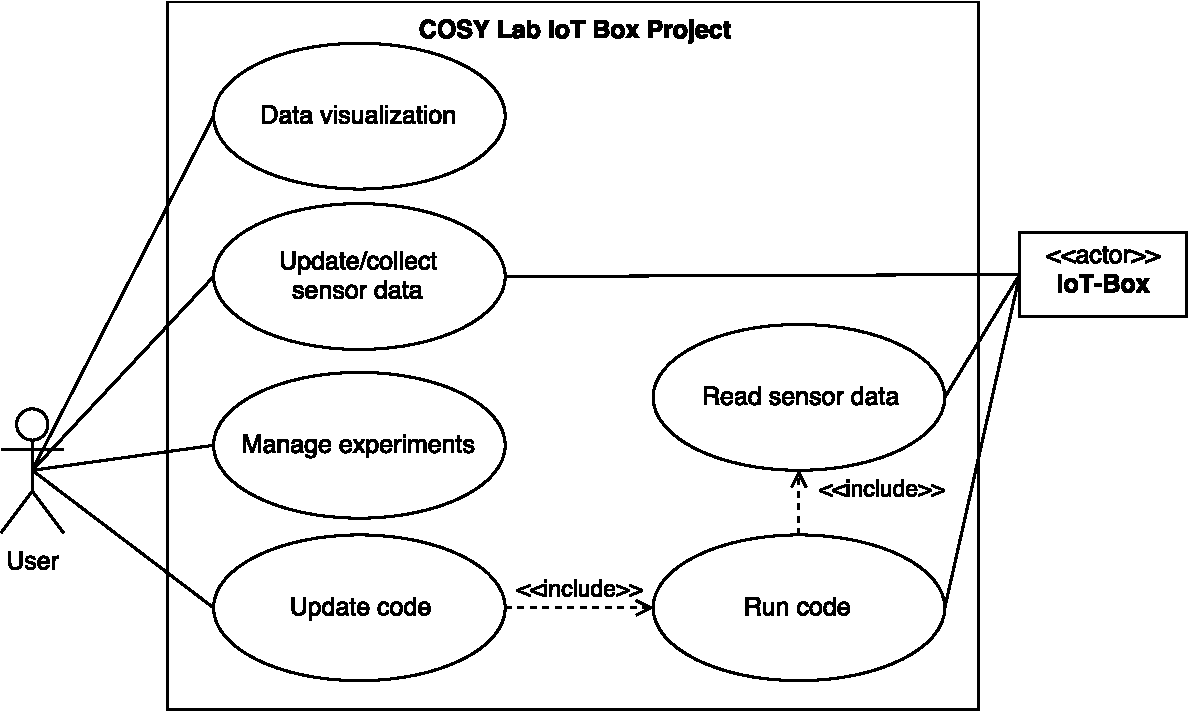
\includegraphics[width=13cm]{Use_Case_Diagram.pdf}
	\caption{Use case diagram describing the \gls{CoSy} Lab \gls{IoT}-Box Project}
	\label{fig:useCase}
\end{figure}

\subsubsection{Manage Experiments}

This use case includes two work flows regarding experiments that are run on one or several \gls{IoT}-Boxes. Experiments in this scope are all installations of the software on the Raspberry Pis. It should be possible to register new experiments and remove ones that are not needed anymore. Also a secure access should be guaranteed in case somebody that is not authorized tries to access this information. In this case the job is completely done by Seattle.

\subsubsection{Update Code}

To adapt to different use cases of the boxes, it will be necessary to update its purpose and code over the Internet. The user is able to upload a code snippet with the functions that he wants to run and decides to push it to one or multiple boxes. Here the user has the choice which sensor data are collected, the interval and the file format it is saved in. After a successful upload the boxes will try to run it and start its data collection or return an error to the user. Access control should also be implemented in this case to allow just authorized users to update code fragments. Seattle also has methods that help with that whole use case.

\subsubsection{Run Code}

Every uploaded code needs to be run by the boxes. It is important to do that so the user is able to collect data from the sensors attached to the box. Depending on the code that is pushed different kind of sensor data can be fetched and saved. This job gets done by Seattle as well.

\subsubsection{Read Sensor Data}

To analyze data they need to be collected first. Over the \gls{I2C} protocol a connection will be established and some sensor data will be fetched. The uploaded code decides which sensors are contacted and the time interval in which new data is appended to a file. Depending on the use case it should be possible to use different sensors that were not thought of at the beginning of this work or are good additions to the existing ones. Because every sensor is different, like newer revisions or different kinds of design and companies, it will be mostly necessary to update the software loaded onto the Raspberry Pis. This process is explained in more detail in Section \ref{implementation}.

\subsubsection{Collect Sensor Data}

It is possible to download the files over the Internet produced by the user supplied code and after some sensor data were read and saved to the boxes. The data that were fetched can be used to plot some graphs using the dedicated homepage that was developed during this work and is described in Section \ref{implementation} and the next use case. Regarding the open data requirement it should be able to publish that data for everybody to download, use, share and work with.

\subsubsection{Data Visualization}

The data visualization is another crucial part of this work. It would also be possible to visualize the data with applications like Excel from Microsoft\footnote{\url{https://products.office.com/de-at/excel}} and similar tools. It would be just necessary to provide the raw data for the end user. On the other hand it is handy to offer the user a tool, or web page in this case, where he can upload his data and the visualization is automatized. Additionally it would be possible to store data on the web server and demonstrate it using the plotting tool that is specially customized to the format and output of the boxes. 

\subsubsection{Alternatives}

Searching for solutions, it was decided that Seattle was a satisfying approach in this case. There were other thoughts and alternatives before Seattle came up though. For example it was an option to built the decentralized system behind it from scratch. Using \gls{IoT} patterns mentioned in \cite{iotPatterns}, like device shadowing for a persistent storage of the data, that would have allowed to reach a device, even if it is offline and unavailable right now. Implementing a rules engine would have helped to dynamically run routines for fetching sensor data if the user sends a particular message to the system. If the boxes would have been used in outdoor places that are not overlooked or secured, it would also have been helpful to have a remote lock feature.

Some of these patterns are already available in the Seattle framework, like a rules engine that supports actions via a special scripting language. Additionally to that, it also covers and solves problems like cluster management and code pushing. It was also decided that building an \gls{IoT} system from scratch would be out of scope for a bachelor project.

\subsection{System Overview - Software Deployment}

The deployment of the software artifacts is divided into three parts. Looking at Figure \ref{fig:deployment} it can be 
differentiated between four different devices: 
\begin{description}
\item["User-Client"]
is typically the home computer of the end user
\item["Web-Server"]
is used for the visualization of the data
\item["Raspberry Pi"]
is part of the subsystem "\gls{IoT}-Box" and executes the user provided code 
\item["Various Sensors"]
are part of the subsystem "\gls{IoT}-Box" and collect data from the environment
\end{description}

\begin{figure}[ht]
	\centering
	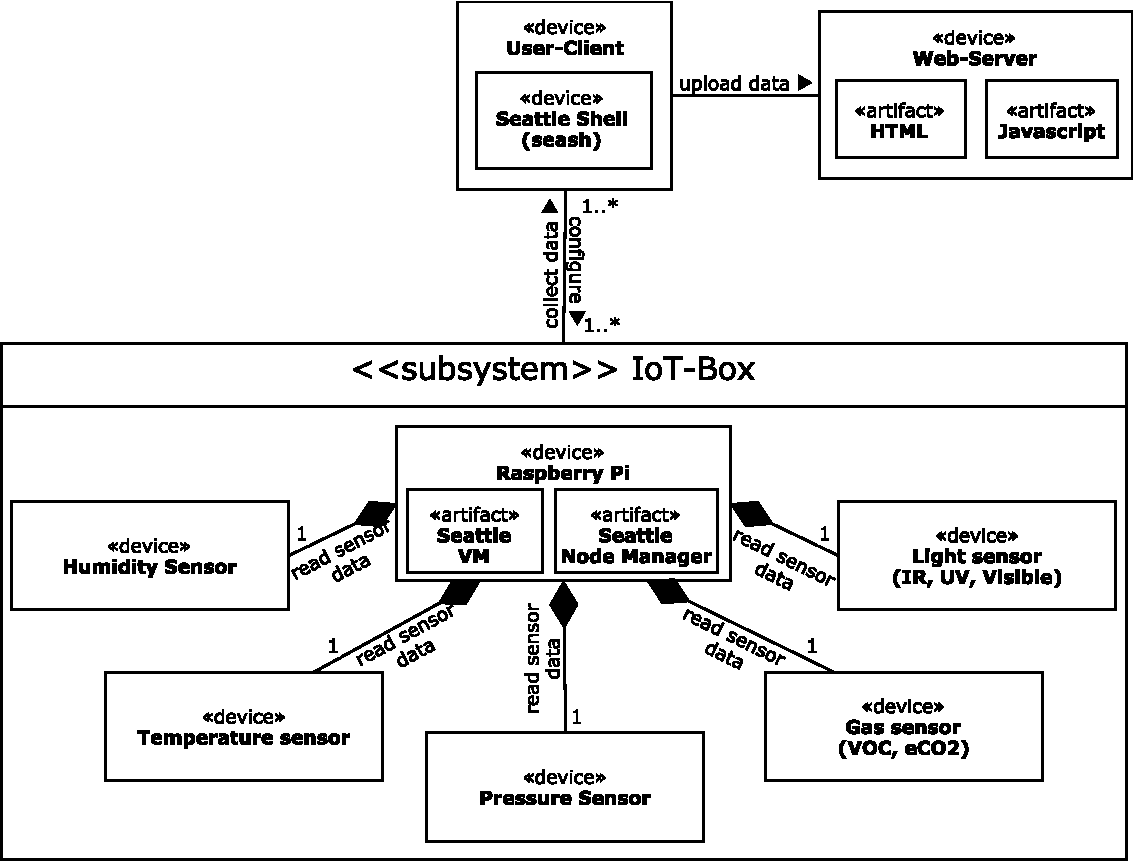
\includegraphics[width=13.5cm]{Deployment_diagram.pdf}
	\caption{Deployment diagram}
	\label{fig:deployment}
\end{figure}

\subsubsection{Raspberrry Pi}

The Raspberry Pi includes parts of the Seattle framework. The Seattle \gls{VM} executes the user provided code and prevents to run malicious content that could break out of the \gls{VM} to get access to the system it is running on. It also prevents the application from using too many resources from components like the \gls{CPU} or memory. \cite[38]{seattlePaper}

The Seattle Node Manager is important for quite a few things. First, it manages access control and allows just authorized parties to execute code on the device it is installed on. At the same time, it provides an interface to upload code, manage a \gls{VM} and download collected data and logs from it. \cite[38]{seattlePaper}

All kinds of different sensors joined with a Raspberry Pi are components of the subsystem "\gls{IoT}-Box". In this case the sensors are a humidity, temperature and pressure sensor, a gas sensor collecting \gls{TVOC} and \gls{eCO2} data, as well as a light sensor for \gls{IR}, \gls{UV} and visible light that are described further in Section \ref{sensorDesc}. Using Seattle allows to have one or many \gls{IoT}-Boxes like this that are configured by one or many authorized User-Clients.

\subsubsection{Web-Server}

The visualization of the data takes place on the Web-Server, or to be precise in fact on the User-Client by processing the JavaScript files that are provided by the server. It is possible to load a file with the sensor data into the script and let it plot different graphs for every available data entry. The output is presented to the user through the web page in his browser. Regarding open data it is also possible to save files on the web server by the administrator to share it with the public.

\subsubsection{User-Client}

Through \gls{seash} it is possible to connect to Raspberry Pis if the user is authorized to do so. The User is able to install \gls{seash} onto his device and configure the \gls{VM}, push code to it, as well as collect the data that are generated through his code. \Gls{seash} operates here as a service manager and allows the interaction with the node manager. The user client also connects to the web server via a browser of his choice and opens up the web page to process his data, that he downloaded from the Raspberry Pis. \cite[38]{seattlePaper}

%%%%%%%%%%%%%%%%%%%%%%%%%%%%%%%%%%%%%%%%%%%%%%%%%%%%%%%%%%%%%%%%%%%%%%%%%%%%%%%%
\section{Implementation} \label{implementation}

There are three parts to the implementation. The first part was the decision of buying several sensors, solder them if necessary, connect them to the Raspberry Pi and test them. The second part consisted of developing the software to operate the sensors and extend Seattle in that way, that it can call those software functions. In the end a home page was built that can be used for visualization and informing other people about the project and progress.

\subsection{Sensor Exploring} \label{sensorDesc}

Looking for different use cases that were not just practical but also useful in the sense of doing research with them, the decision was made to buy three different sensors. In combination they were collecting useful data about the environment that could be used in all rooms of a home, in a lab and outdoors for example. Furthermore all sensors are breakout boards by the company Adafruit\footnote{\url{https://www.adafruit.com/}} and it was necessary to solder the header onto the \gls{PCB}. It was also required that all sensors support the \gls{I2C} protocol.

\subsubsection{Temperature, Barometric Pressure and Humidity Sensor} 

The first thing that comes to mind when talking about environment is the temperature. After all it is something that we experience ourselves everyday. Combined with measuring barometic pressure, also known as atmospheric pressure, and humidity it is a suitable addition to the \gls{IoT}-Box. The BME280 environmental sensor was manufactured by Bosch\footnote{\url{https://www.bosch-sensortec.com/}} and has an accuracy of \pm3\% regarding humidity, \pm1 \gls{hPa} with barometic pressure and \pm1.0°\gls{C} with temperature. \cite{bme280}

Additionally, The company STMicroelectronics\footnote{\url{http://www.st.com/}} sponsored sensors from their product line. For one, the HTS221 for relative humidity and temperature and the LPS25HB for absolute pressure was sent to support the project. They have an accuracy of \pm0.5°\gls{C} regarding temperature between 15°\gls{C} and 40°\gls{C}, \pm3.5\% with humidity and \pm1 hPa  with barometic pressure. \cite{stHum} \cite{stPress}

\subsubsection{Light Sensor} 

Knowing the \gls{UV} index is sometimes quite a useful information, like when you're outside a lot on a hot summer day or when you just want to do some measurements. The SI1145 light sensor from SiLabs\footnote{\url{https://www.silabs.com/}} calculates the \gls{UV} index based on the \gls{IR} and visible light from the sun. As a side note, these last two values have no units to them, because they are based on the light that is falling onto them.  \cite{si1145}

\subsubsection{Air Quality Sensor} \label{sec:airQual}

There is a lot of air pollution in big cities that is harmful to every person if it is present in high amounts. Especially in the morning when people drive to work with cars the \gls{CO2} pollution is increasing immensely \cite{carWork}. To measure that, it was decided to get an air quality sensor - the CCS811. The chip was developed by the company ams\footnote{\url{http://ams.com/}} and collects \gls{eCO2} and \gls{TVOC} data. It has a range from  400 to 8192 \gls{ppm} regarding \gls{eCO2} and 0 to 1187 \gls{ppb} with \gls{TVOC}. It is also recommended to run it 48 hours after buying it to burn it in and always start to read data 20 minutes after beginning the sensor reading. Unfortunately, after starting the data collection for the evaluation it was clear that the air quality sensor does not work properly with the Raspberry Pi because the sensor uses clock stretching that the Pi does not support. \cite{ccs811}

\subsection{Software Development}

The next step taken after connecting the sensors to the Raspberry Pi over the \gls{I2C} dedicated Pins was to develop software classes and extend the Seattle \gls{Repy} V2 code to be able to call the functions in these classes. Figure \ref{fig:classDiagram} shows a small excerpt of these classes that are described in the following sections as well.

\begin{figure}[ht]
	\centering
	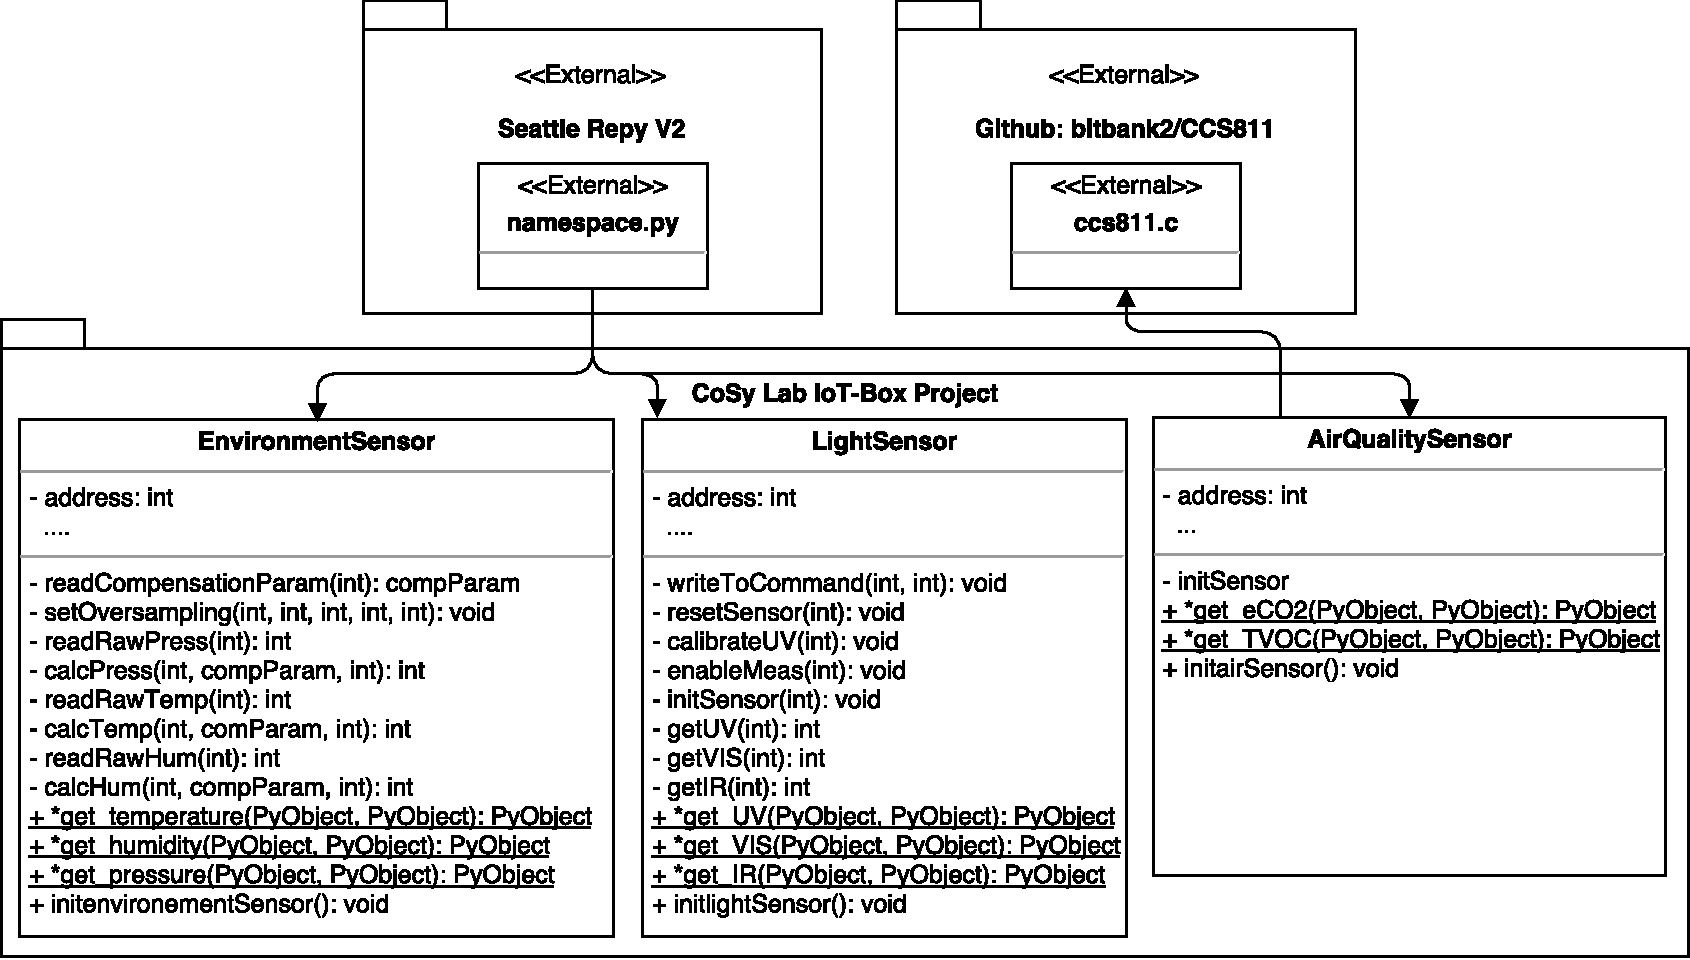
\includegraphics[width=13.5cm]{Class_Diagram_Cropped.pdf}
	\caption{Excerpt of the class diagram}
	\label{fig:classDiagram}
\end{figure}

\subsubsection{Writing the Classes}

At the first meeting there was a discussion about the programming language that would be used for this project. The decision was between Python\footnote{\url{https://www.python.org/}}, Java\footnote{\url{https://java.com/}} and C. Seattle is programmed using the Python language. It was therefore a good choice for this situation. Consequently, it was inevitable to use a wrapper if Java or C code would be used to extend the existing Seattle code base. 

The "Computer Language Benchmark Game" made it their goal to benchmark different programming languages with several programs. Looking at the performance at \cite{speedComp}, then it becomes clear that C is the fastest of all these languages. Not far after that, there is Java with less than three seconds difference. Far behind is Python with ten and up to almost 100 seconds run time. After all, it depends on the program that is being executed. Some programming languages do the job more quickly and effective than others. In \cite[54]{pythonC}, there is a runtime comparison between Python, C and Python extended with C. There is a big improvement of the factor ~25 (431.42/17.05) between just Python and the one extended by C if the program from \cite{pythonC} is run 500 times.

The decision was also made based on a personal preference. Being more in contact with Java and C through internships and courses at the university, it was easier to perform this project with the already available know-how. Looking for available resources online, there was an official section in the documentation of Python about extending it with C\footnote{\url{https://docs.python.org/2/extending/extending.html}}, as well.

\subsubsection{Extending Seattle with C}

On the basis of the previous information it was an appropriate solution to 
go with the programming language C. Drivers were written with the help of the documentations from the sensors that were attached to the Raspberry Pi and resources found on the Internet. After testing them on the device itself and checking that the right values were returned, a shared library and Python module was created using the \gls{GCC}. For example, a shell command could look like that:

\begin{lstlisting}[language=bash,caption={build command for a shared library},captionpos=b]
gcc -shared -Xlinker -export-dynamic -o environmentSensor.so 
-I/usr/include/python2.7/ -lpython2.7 -lwiringPi 
BME280_TempSensor.c
\end{lstlisting}

In this case a shared library is created with the parameters "-shared -Xlinker -export-\\dynamic". The output file would be "environmentSensor.so" and the input file is the C class "BME280\_TempSensor.c". The WiringPi and Python libraries and imports are necessary to build the class properly.
The .so file, that is produced calling that command, can be loaded into Python as a module now. Visible are just special functions though. Looking at Figure \ref{fig:classDiagram}, the static functions that return the PyObject are added in the init function (like initenvironmentSensor()) so that Python is able to work with them.

Having a working Python module available, it was now possible to extend Seattle with that code. The modules were added to the \gls{Repy} \gls{SB} by expanding the \gls{API} with the specific function calls, like get\_temperature. This was done in the namespace.py file (see Figure \ref{fig:classDiagram}). The extended \gls{Repy} V2 source code is available online at \cite{repyFork}.

All of that work allows the user in the end to call the functions through \gls{seash} over the Internet. The message flow when running the \gls{Repy} code provided by the user is illustrated in Figure \ref{fig:cPython}. Here the experiment calls the \gls{API} in the \gls{Repy} \gls{SB} that runs the Python code. At that point, it was possible to call a Python module, a less preferred way to execute Popen to use Shell-Tools or in this case through the CPython \gls{API} the C code is executed and accesses the \gls{I2C} messages through the wiringPi library. The values are then returned to the experiment where it is being processed.

\begin{figure}[ht]
	\centering
	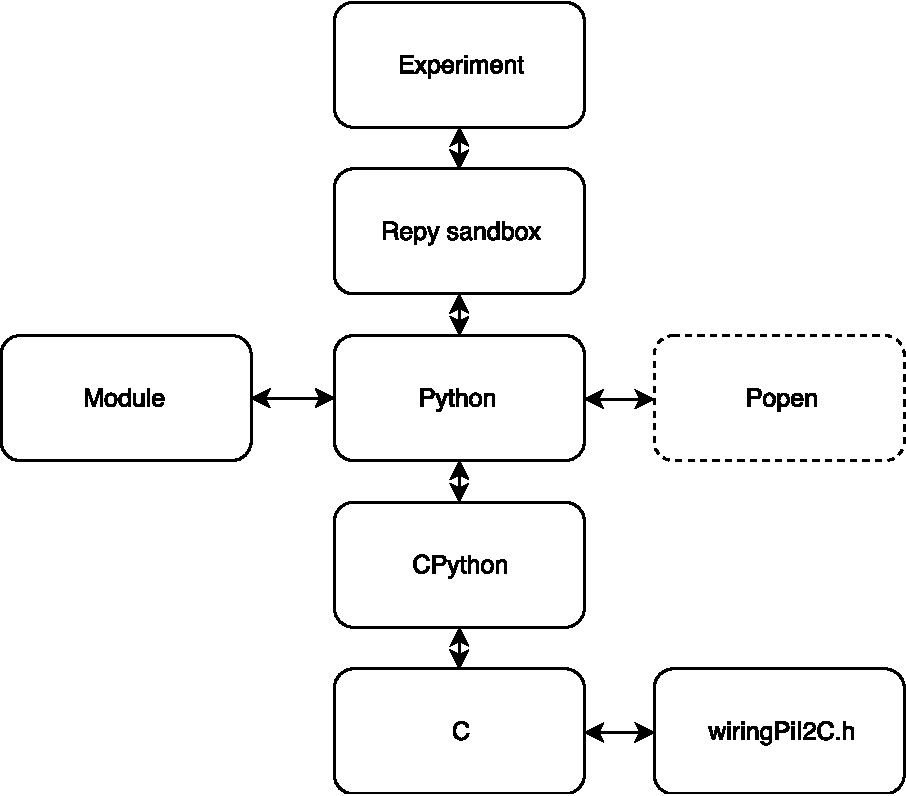
\includegraphics[width=9cm]{CPython_Workflow.pdf}
	\caption{Path from experiment to C code}
	\label{fig:cPython}
\end{figure}

\subsection{Visualization and Homepage}

The last part of the implementation was the homepage to visualize the data. The goal of the homepage was to provide the user with a way to visualize his data and to have a platform to inform about other information regarding the boxes as well as developments.

The website, that is visible in Figure \ref{fig:homepage}, uses various libraries and frameworks to offer those features. First and foremost the design and front-end was accomplished using Bootstrap\footnote{\url{https://getbootstrap.com/}}, dependent on that JQuery\footnote{\url{https://jquery.com/}} is necessary, too, and last but not least Font Awesome\footnote{\url{https://fontawesome.com/}} for various kinds of icons. Since Bootstrap is able to optimize a web page for both mobile and desktops, it is able to view this homepage on most modern devices with multiple screen resolutions. As a side note the homepage is just there to showcase the visualization and provide a template for others therefore there is just one web page available as of now.

To plot the charts the JavaScript library Angular-nvD3\footnote{\url{http://krispo.github.io/angular-nvd3/}} was used. This library depends on a few other ones. As the name states Angular\footnote{\url{https://angular.io/}}, NVD3\footnote{\url{http://nvd3.org/}} and D3.js\footnote{\url{https://d3js.org/}} are required to be loaded, too. They are the back-end of this homepage and are responsible to build the charts using the data uploaded by the user.

First the user is asked to upload a file. That file needs to be in \gls{JSON} format\footnote{\url{https://www.json.org/}}. The function that processes the file searches for a specific key and adds the value and date to the corresponding chart. The available keys that were used in this project are:

\begin{itemize}
  \setlength\itemsep{0em}
  \item Time
  \item Temperature
  \item Humidity
  \item Pressure
  \item UV
  \item IR
  \item VIS
  \item eCO2
  \item TVOC
\end{itemize}

\begin{figure}[ht]
	\centering
	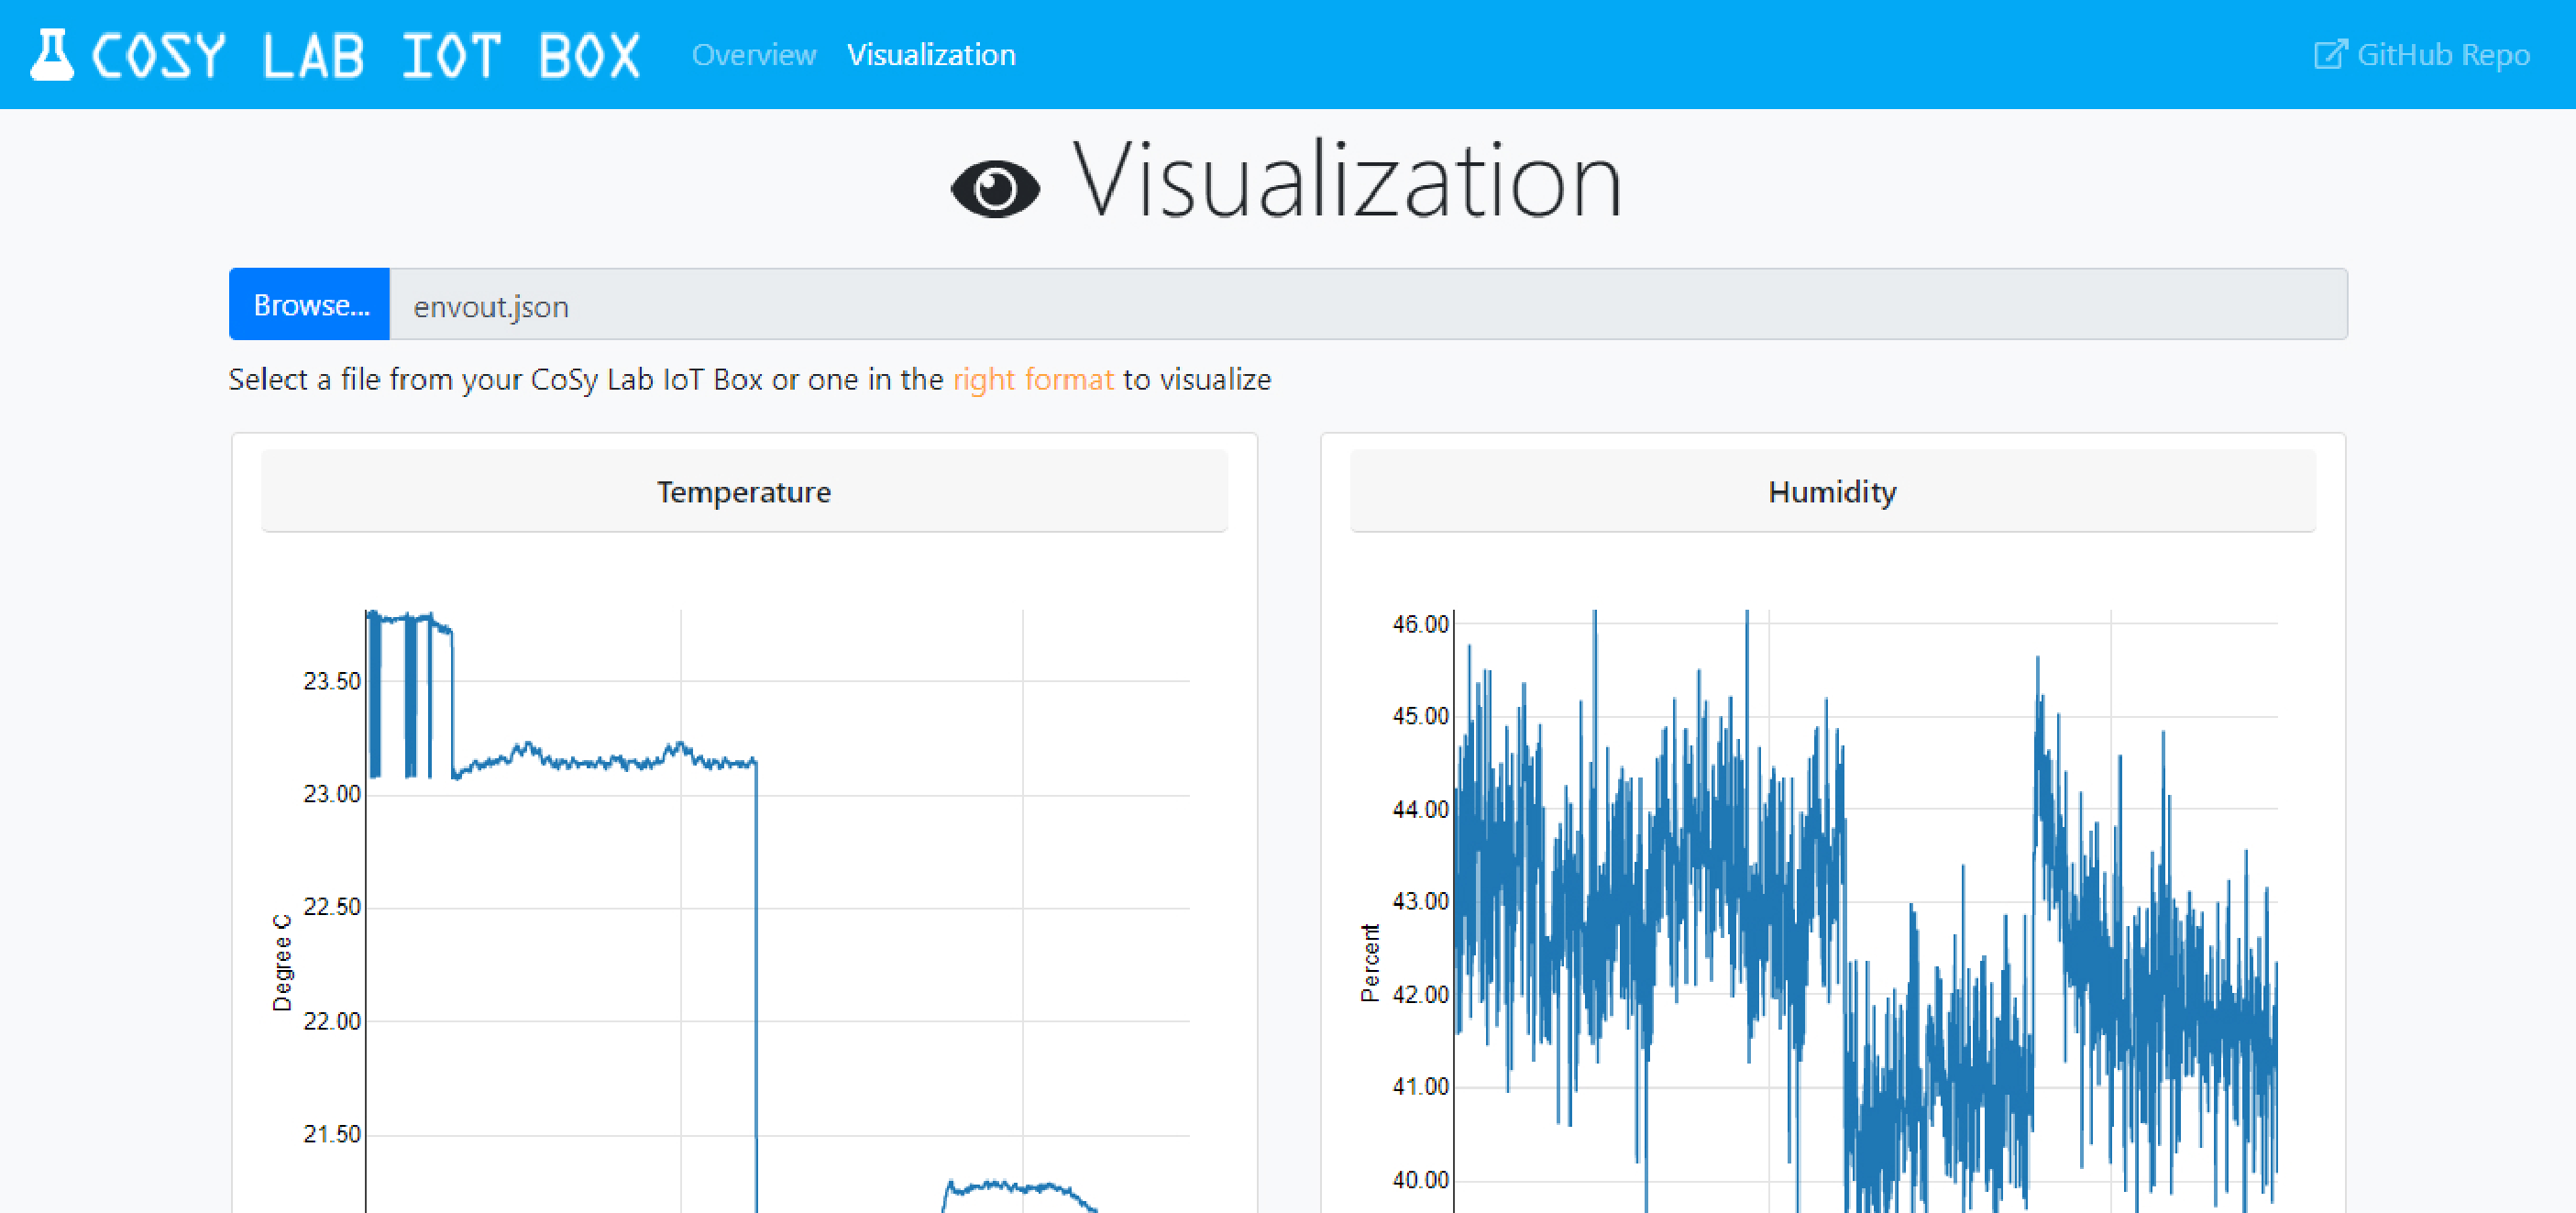
\includegraphics[width=13.5cm]{Website_Mockup.pdf}
	\caption{Screenshot of the visualization homepage}
	\label{fig:homepage}
\end{figure}

The whole collection of key-value pairs is iterated and pushed into the values array of the charts. The charts are refreshed through the \gls{API} from Angular-nvD3 after the last task is finished. That process after uploading the file normally takes just a few seconds and depends on the amount of values being inserted.

%%%%%%%%%%%%%%%%%%%%%%%%%%%%%%%%%%%%%%%%%%%%%%%%%%%%%%%%%%%%%%%%%%%%%%%%%%%%%%%%
\section{Evaluation	and	Testing}

Many use cases are possible with the \gls{IoT}-Box and there are plenty of possibilities to extend it with available sensors on the market. Therefore it is not easy to test the box for every eventuality but at least some evaluation and testing can be done for the most probable utilization of it.

\subsection{Functional Evaluation}

Working with the box for the last weeks and months there were some work flows that repeated themselves quite a lot. Based on that a use case scenario was created:

\subsubsection*{\textbf{Use Case Scenario - Collecting Data and Visualizing it}}

\begin{itemize}
  \setlength\itemsep{0em}
  \item John Doe successfully connects over \gls{seash} with his cluster of \gls{IoT}-Boxes with his personal key
  \item John prepared a \gls{Repy} code that he now uploads to the boxes and starts them
  \item After a while John stops the execution of his code and downloads the files that were created during that time
  \item Fortunately, John saved all those collected values in one JSON file and has now temperature, humidity, pressure, \gls{UV}, \gls{IR}, visible light, \gls{eCO2} and \gls{TVOC} data that he uploads to the web page
  \item The web page processes his file and plots graphs for them that John can analyze
\end{itemize}

Some tests were conducted on the basis of this use case scenario that are visible in Table \ref{tab:funcTest}. Not everything was tested because some functions are already implemented in Seattle and were not worked on as part of this work, like up- and downloading files to the boxes for example.

Most of the tests worked well and satisfying. The partial result with the long-term experiment is connected with the other two partial results. As mentioned in Section \ref{sec:airQual} the air quality sensor does not fully work with the Raspberry Pi. It was just possible to collect data for a shorter period of time than with the others. The other sensors worked properly as we see in Table \ref{tab:funcTest}. A long-term experiment is therefore possible if the sensor is not used.

\begin{table}[H]
\centering
\begin{tabular}{|l|l|}
\hline
\textbf{Test} & \textbf{Result} \\ \hline
Doing a long-term experiment & Partial \\ \hline
Reading temperature & Worked \\ \hline
Reading humidity values & Worked \\ \hline
Reading pressure values & Worked \\ \hline
Reading \gls{UV} values & Worked \\ \hline
Reading \gls{IR} values & Worked \\ \hline
Reading visible light values & Worked \\ \hline
Reading \gls{eCO2} values & Partial \\ \hline
Reading \gls{TVOC} values & Partial \\ \hline
Visualizing collected data & Worked \\ \hline
\end{tabular}
\caption{Tested features of the \gls{IoT}-Box implementation}
\label{tab:funcTest}
\end{table}

\subsection{Experiment Evaluation}

For the experiment the \gls{IoT}-Box was put at the window during winter time in Vienna, on the 09.02.2018 to be exact. According to WetterOnline\footnote{\url{https://www.wetteronline.at/wetterdaten/wien}}, the outdoor temperature at "Hohe Warte" was between 0°\gls{C} and 3°\gls{C}. humidity was measured at 74\% and pressure at 1019 \gls{hPa}. The \gls{IoT}-Box collected data for several hours before the files were downloaded through \gls{seash}. Having the file at hand, it was loaded into the visualization web page to create some charts.
\newpage

First we have the temperature in Figure \ref{fig:evalTemp}. At 7 in the morning the heating started and the temperature has risen up to its peak at 13:15 with 20.30°\gls{C}. At 15 the window was opened for 30 minutes and the temperature fell 2°\gls{C} before it rises up again a bit. The lowest point was reached at 4:40 am with 18.42°\gls{C}. The mean is 19.43 from all 2000 collected values.

The humidity in \ref{fig:evalHum} did not change much. It started at midnight with 56.89\% humidity and in the end just raised by less than 6\% at 62.34\%, its peak. The lowest point was at 7:50 am with 50.55\% and the mean is 55.24\%. Opening the window also pumped up the humidity a small amount to compensate the change between outside and the room.

Comparing the pressure with the information from WetterOnline it is apparent that it was climbing that day. That also reflects with the values recorded by the box. Starting at 979.39 \gls{hPa} that numbers grows up to 985.77 \gls{hPa}.

\begin{figure}
\begin{subfigure}[c]{0.5\textwidth}
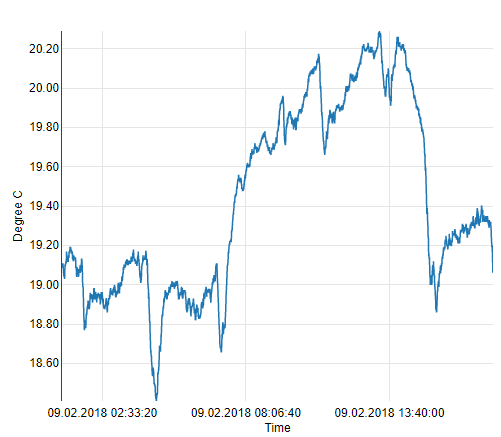
\includegraphics[width=1\textwidth]{expEval/Temp_09-02-2018.PNG}
\subcaption{Temperature data (in \gls{C})}
\label{fig:evalTemp}
\end{subfigure}
\begin{subfigure}[c]{0.5\textwidth}
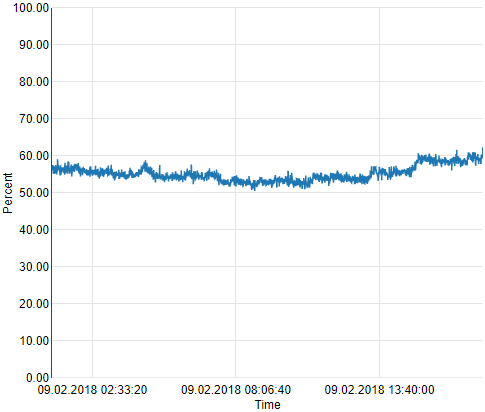
\includegraphics[width=1\textwidth]{expEval/Hum_09-02-2018.PNG}
\subcaption{Humidity data (in \%)}
\label{fig:evalHum}
\end{subfigure}
\par\medskip
\begin{subfigure}[c]{\textwidth}
\centering
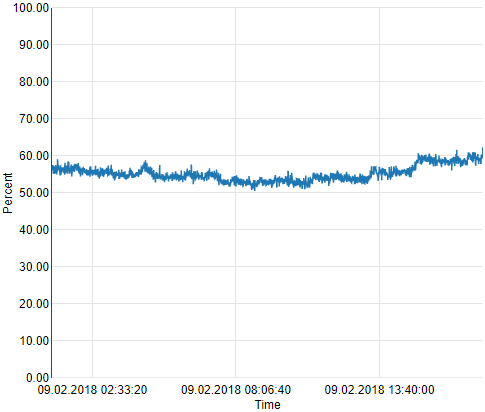
\includegraphics[width=0.5\textwidth]{expEval/Hum_09-02-2018.PNG}
\subcaption{Pressure data (in \gls{hPa})}
\label{fig:evalPres}
\end{subfigure}
\caption{Data collected by the BME280 sensor}
\end{figure}

That day the sun did not shine very bright. Inspecting Figure \ref{fig:evalIR} and \ref{fig:evalVIS} we can see that the sunrise was at 7 in the morning. Looking at the graphs we can see that there are no units because the sensor just measures how many light falls into it. Therefore it is just there for information but using those two values it is possible to calculate the \gls{UV} index that we see in Figure \ref{fig:evalUV}. That day it stayed under two. That is a pretty low value and not harmful for the normal human skin. 

\begin{figure}
\begin{subfigure}[c]{0.5\textwidth}
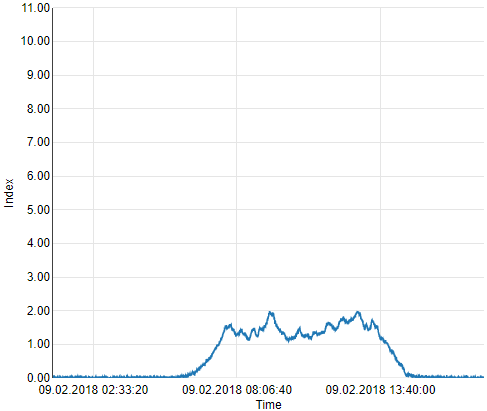
\includegraphics[width=1\textwidth]{expEval/UV_09-02-2018.PNG}
\subcaption{\gls{UV} data (index)}
\label{fig:evalUV}
\end{subfigure}
\begin{subfigure}[c]{0.5\textwidth}
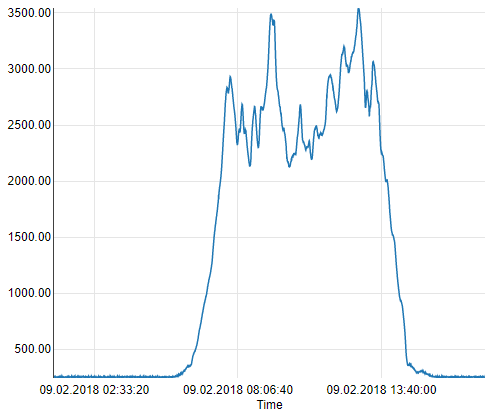
\includegraphics[width=1\textwidth]{expEval/IR_09-02-2018.PNG}
\subcaption{\gls{IR} light data}
\label{fig:evalIR}
\end{subfigure}
\par\medskip
\begin{subfigure}[c]{\textwidth}
\centering
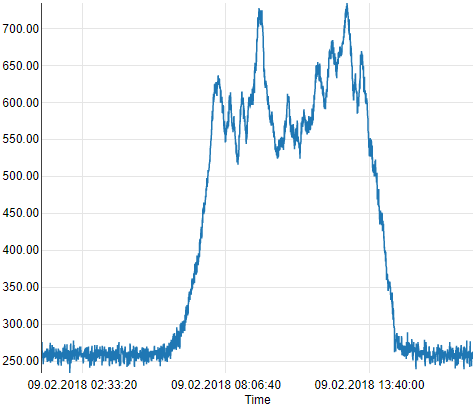
\includegraphics[width=0.5\textwidth]{expEval/VIS_09-02-2018.PNG}
\subcaption{Visible light data}
\label{fig:evalVIS}
\end{subfigure}
\caption{Data collected by the SI1145 sensor}
\end{figure}

%After the 20 minutes burn in that is necessary for the sensor to calibrate correctly it started to measure some data. During the day the \gls{eCO2} and \gls{TVOC}

\begin{figure}
\begin{subfigure}[c]{0.5\textwidth}
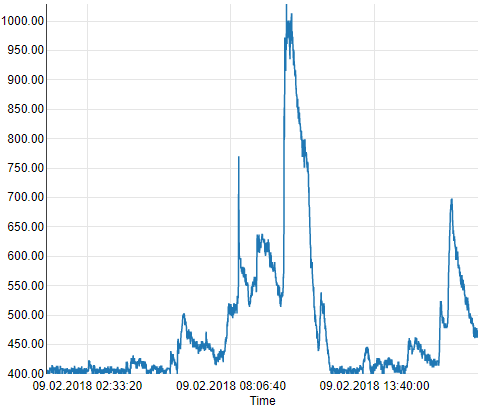
\includegraphics[width=1\textwidth]{expEval/eCO2_09-02-2018.PNG}
\subcaption{\gls{eCO2} data}
\label{fig:evalCO2}
\end{subfigure}
\begin{subfigure}[c]{0.5\textwidth}
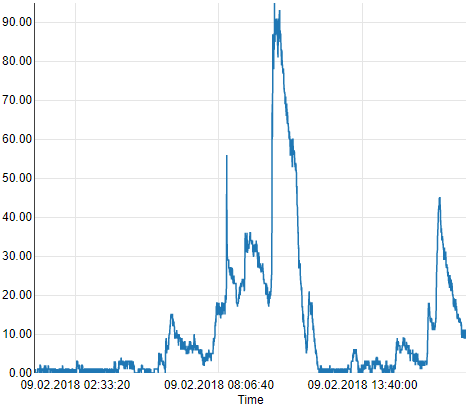
\includegraphics[width=1\textwidth]{expEval/VOC_09-02-2018.PNG}
\subcaption{\gls{TVOC} data}
\label{fig:evalTVOC}
\end{subfigure}
\caption{Data collected by the CCS811 sensor}
\end{figure}

%%%%%%%%%%%%%%%%%%%%%%%%%%%%%%%%%%%%%%%%%%%%%%%%%%%%%%%%%%%%%%%%%%%%%%%%%%%%%%%%
\section{Conclusion}

The solution approach presented in this work is combining Seattle with the Raspberry Pi to build a network of \gls{IoT} devices and grab the sensor data off them that they were collecting. After working with that setup for several weeks, it emerged, that the advantages of Seattle with its cluster management, code pushing, the \gls{SB} and extendability of the API with just a few lines of code made it the suitable candidate as a software base. The flexibility of that approach made that solution more future proof because new sensors can be attached and used with the existing ones.

During the implementation there were no bigger problems that came up. The only negative development was the sensor not working properly with the Raspberry Pi. As already described in the functional evaluation, it was still possible to operate with it but not in the way it was intended. That was a small drawback regarding the full functionality of the \gls{IoT}-Box but it is fixable quite quickly by replacing the sensor with another one.

Additionally, it is just possible to configure the \gls{IoT}-Boxes over the Internet. They need a working connection so that the user can upload and start his file through \gls{seash}. On the other hand it also simplifies the process of configuring multiple boxes at once.

\subsection{Future Work}

In the future it would be possible to expand the sensor diversity. There are a lot of different sensors for sale like motion, sound, GPS and plenty more. Even sensors that have not been developed yet and are just future thinking could possibly be paired with a Raspberry Pi which has Seattle installed. 

To conduct some outdoor research, it would be helpful to have a support for LoRa and LoRaWAN \cite{lora}. LoRaWAN is based on LoRa and is able to store data in a database over a long distance by uploading them through a gateway. An application server like the visualization web page for example could fetch the data and have an up-to-date collection of charts.

%%%%%%%%%%%%%%%%%%%%%%%%%%%%%%%%%%%%%%%%%%%%%%%%%%%%%%%%%%%%%%%%%%%%%%%%%%%%%%%%
\printbibliography[heading=bibintoc]

%\section{Appendix}

\end{document}
